\section{Experiments}

\vspace{-0.05in}
We validate our  algorithmic insights and then our theory.
In Section \ref{sec_exp_res}, we first show that single-task learning results can help predict positive or negative transfer.
%the single-task based metric on sentiment analysis and ChestX-ray14 datasets.
Second, our proposed incremental training schedule improves the training efficiency of standard multi-task training on sentiment analysis tasks.
%Third, we measure the data efficiency ratio of multi-task learning on six sentiment analysis tasks.
In Section \ref{sec_exp_ab}, we validate our theoretical results.
We further show that when the sample ratio is large, performing the alignment procedure of \cite{WZR20} provides more improvement for MTL.

\begin{table}[!b]
\begin{minipage}[t]{.58\textwidth}
	\vspace{-0.1in}
	\centering
  \begin{tabular}{c c c c c}
	\toprule
		\multirow{2}{*}{{\bf Threshold}}  & \multicolumn{2}{c}{{\bf Sentiment
		analysis}} & \multicolumn{2}{c}{{\bf ChestX-ray14}} \\
		& Precision &  Recall & Precision &  Recall \\
		\cmidrule(lr){1-1} \cmidrule(lr){2-3} \cmidrule(lr){4-5}
		0.0 & 0.596 & 1.000 & 0.593 & 1.000 \\
		0.1 & \textbf{0.756} & \textbf{0.388} & \textbf{0.738} & \textbf{0.462} \\
		0.2 & 0.919 & 0.065 & 0.875 & 0.044 \\
		% 0.3 & 1.000 & 0.004 &     - &     - \\
	\bottomrule
	\end{tabular}
	\vspace{0.1in}
	\captionof{table}{Single-task learning results can help predict postive or negative transfer in multi-task learning.}
	\label{tab:mtl_better_than_stl}
\end{minipage}%
\quad
	\begin{minipage}[t]{.40\textwidth}
	\vspace{-0.1in}
	\centering
	\begin{tabular}{c c c}
		\toprule
		% \multirow{2}{*}{{\bf Models}} & \multicolumn{2}{c}{\begin{minipage}{1.2in}\begin{center}
		% Sentiment\\ analysis\end{center}\end{minipage}} \\
		\multirow{2}{*}{{\bf Models}} & \multicolumn{2}{c}{\bf Sentiment analysis} \\
		% \cmidrule(lr){2-3}
		& all tasks & w/o TREC \\
		\midrule
		{\bf MLP}  & 31\% & 29\% \\
		{\bf LSTM} & 35\% & 34\% \\
		{\bf CNN}  & 30\% & 28\% \\
		\bottomrule
		\end{tabular}
	\vspace{0.1in}
	\captionof{table}{Efficiency of incremental training compared to baseline MTL.}
	\label{tab:taskonomy}
\end{minipage}
\end{table}

\vspace{-0.07in}
\subsection{Experimental Setup}

We consider a text classification task and an image classification task as follows.

{\it Sentiment Analysis.} We consider six tasks: movie review sentiment (MR) \cite{pang2005seeing}, sentence subjectivity (SUBJ) \cite{pang2004sentimental}, customer reviews (CR) \cite{hu2004mining}, question type (TREC) \cite{li2002learning}, opinion polarity (MPQA) \cite{wiebe2005annotating}, and the Stanford sentiment treebank (SST) tasks \cite{socher2013recursive}.
%The question is to predict positive or negative sentiment expressed in the text.
We use an embedding layer with GloVe embeddings \cite{pennington2014glove}
followed by an LSTM, MLP or CNN layer proposed by~\cite{lei2018simple}.

%multi-layer perceptron (MLP), LSTM, CNN on all tasks
%We use this task to verify our theoretical results on model capacity and task covariance in real world.

{\it ChestX-ray14.} This dataset contains 112,120 frontal-view X-ray images \cite{chexnet17}.
There are 14 diseases (tasks) for every image that we would like to predict.
We use densenet121 as the shared module \cite{huang2017densely}.
%We treat each label as one task a binary classification problem and formulate it as a 14-task multi-task learning problem.
%This dataset is curated where the labels
%We use the CheXNet model from~\cite{chexnet}, which is a 121-layer convolutional neural network on all tasks.


%\textbf{The training procedure and baseline.}
For all models, we use a shared module for all tasks and assign a separate output layer on top of the shared module for each task.
The baseline training schedule for MTL is the round-robin training schedule.
%We compare our incremental training schedule of Algorithm \ref{alg_inc_train} to the round-robin training schedule.
We measure the test accuracy of predicting a target task.
We measure computional cost by summing over all epochs the number of samples used in every epoch.

\vspace{-0.07in}
\subsection{Experimental Results}\label{sec_exp_res}

\textit{Predicting transfer effect via STL results.}
We show that the single-task based metric proposed in Section \ref{sec_similarity} can predict positive or negative transfer in MTL.
A common challenge in the study of MTL is that the results can be hard to understand.
It is difficult to predict when MTL performs well without running extensive trials.
Our insight is that we can use STL results to help understand MTL results.
Table \ref{tab:mtl_better_than_stl} shows the result on both the sentiment analysis and the ChestX-ray14 tasks.
We find that using a threshold of $\tau = 0.1$, the STL results correctly predict positive or negative transfer with $75.6\%$ precision and $38.8\%$ recall among $30$ times $5$ (random seeds) task pairs!
We observe similar results for $91$ task pairs from the ChestX-ray14 dataset.
%The results show that STL results are indicative of MTL results.

\textit{Mitigating negative transfer via incremental training.}
First, we show that our proposed incremental training schedule (Algorithm \ref{alg_inc_train}) can help mitigate negative transfer for predicting a particular target task.
Over all $15$ pairs from the sentiment analysis tasks, we find that Algorithm \ref{alg_inc_train} requires only $45\%$ of the computational cost to achieve similar performance on the target task, compared to the MTL baseline.
Our insight is that since adding more samples from the source task does not always help, we can improve efficiency by adding source samples \textit{incrementally} during training.

%\textbf{Improving transfer learning training efficiency.}
%We show that Algorithm \ref{alg_inc_train} also applies to transfer learning settings.
%Compared to fine-tuning the source model on the target task, we show that our proposed method reduces the computional cost by \alert{$xx\%$}, without sacrificing accuracy.

Our next result shows the incremental training schedule applies to multiple tasks as well.
In Table \ref{tab:taskonomy}, we find that over all six sentiment analysis tasks, incremental training requires less than $35\%$ of the computational cost compared to baseline MTL training, while achieving the same accuracy averaged over all six tasks.
As a further validation, excluding TREC, we observe similar comparative results.
%The data efficiency ratio of using MLP is $100\%$ because the average performance of MTL is worse than the average of STL.
%We further show that applying incremental training helps reduce the data efficiency ratio to \alert{$xx\%$}.
%If TREC is not included, we see that only $25\%$ of the labeled data is needed.


\begin{figure}[!t]
	\centering
	\begin{subfigure}[b]{0.33\textwidth}
		\centering
		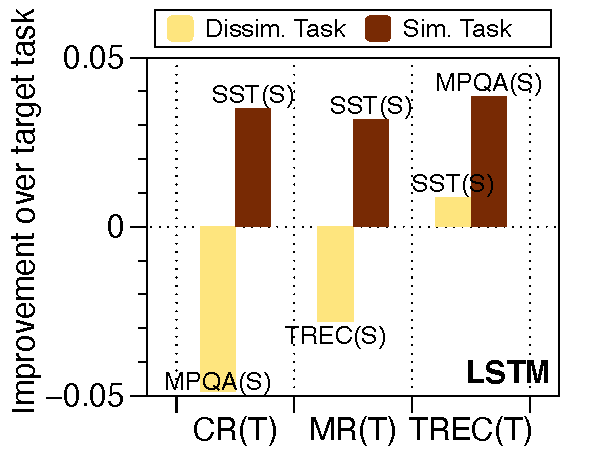
\includegraphics[width=0.975\textwidth]{figures/task_sim_norm_lstm.pdf}
		\caption{Task similarity}
		\label{fig_ab_sim}
	\end{subfigure}%
	\begin{subfigure}[b]{0.33\textwidth}
		\centering
		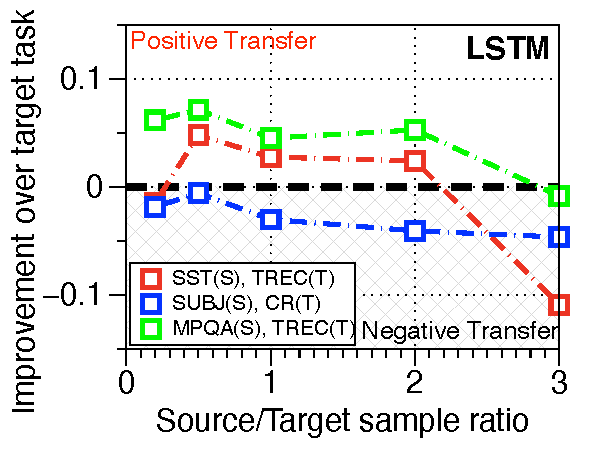
\includegraphics[width=0.975\textwidth]{figures/ratio_norm_3_pairs_lstm.pdf}
		\caption{Sample size}
		\label{fig_ab_data}
	\end{subfigure}
	\begin{subfigure}[b]{0.33\textwidth}
		\centering
		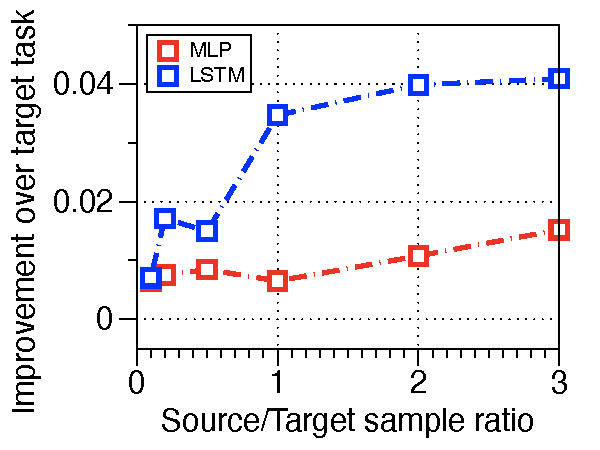
\includegraphics[width=0.975\textwidth]{figures/ratio_alignment_norm_diff_all.pdf}
		\caption{Covariate shift}
		\label{fig_ab_cov}
	\end{subfigure}
	\caption{Validating the three results of Section \ref{sec_insight} on sentiment analysis tasks. (a) Adding a semantically similar source task in MTL performs better than adding a dissimilar task.
	(b) As source/target sample ratio increases, we observe a transition from positive to negative transfer.
	(c) As source/target sample ratio increases, aligning task covariances \cite{WZR20} improves more over the baseline.
	Note: (S) denotes the source task and (T) denotes the target task.}
	\label{fig_ablation}
	\vspace{-0.15in}
\end{figure}

\vspace{-0.07in}
\subsection{Validating the Theoretical Results}\label{sec_exp_ab}

We first validate our theoretical results in Section \ref{sec_similarity} and \ref{sec_data_size}.
In Figure \ref{fig_ab_sim}, we compare the performance training with a semantically similar task versus a dissimilar task with a target task.
We select each task pair based on our domain knowledge.
We observe that adding a similar task helps the target task whereas adding a dissimilar task hurts.
In Figure \ref{fig_ab_data}, we validate that adding more source samples does not always improve performance on the target task.
Finally, we validate the algorithmic consequence of Section \ref{sec_covshift}.
In Figure \ref{fig_ab_cov}, we measure the performance gains from performing the alignment procedure proposed in \cite{WZR20} minus baseline MTL.
We average the results over all 15 task pairs.
The result shows that as the source samples increases, the alignment procedure shows a bigger improvement over MTL.
The rest of experimental procedures are left to Appendix \ref{app_it}.


